\documentclass{article}
\usepackage[T2A]{fontenc} % Загрузка кириллической и стандартной кодировки шрифта
\usepackage[utf8]{inputenc}   % Объявление поддержки UTF-8
\usepackage[russian,english]{babel} % Загрузка поддержки русского и английского языков
\usepackage[letterpaper,top=2cm,bottom=2cm,left=2cm,right=2cm,marginparwidth=1.75cm]{geometry}
\usepackage{graphicx}
\usepackage{caption}
\usepackage{amsmath}
\usepackage{fancyhdr}
%\usepackage{amsfonts} 
\usepackage{hyperref}
\usepackage{microtype}

\usepackage{amssymb}

\newcommand{\sus}[1]{\addcontentsline{toc}{section}{ \small #1}}
\newcommand{\subs}[1]{\addcontentsline{toc}{subsection}{ \small #1}\fancyhead[L]{#1}}
\newcommand{\ssubs}[1]{\subsubsection*{#1}\addcontentsline{toc}{subsection}{ \small #1}\fancyhead[R]{#1}}
\newcommand{\zz}{\newline\newline}
\newcommand{\op}[1]{\textbf{Определение #1} }
\newcommand{\ttt}[1]{\underline{\textit{#1}}}
\newcommand{\nl}{\newline}
\newcommand{\cd}{$\cdot$}
\newcommand{\bb}[1]{\mathbb{#1}}
\newcommand{\ff}[1]{\mathbf{#1}}
\newcommand{\eq}[1]{\begin{equation} #1 \end{equation}}



\title{programming}
\author{Богдан Аленович Руденко}
\date{November 2022}

\begin{document}

\begin{titlepage}
\centerline{Государственный астрономический институт имени П.К. Штернберга}
\centerline{Московский государственный университет имени М.В. Ломоносова}
\centerline{Физический факультет}
\vspace{6cm}
\vspace{2cm}
\centerline{\huge Специальный астрономический практикум}
\vspace{2cm}
\centerline{\huge Основные понятия космологии}
\vspace{0.5cm}
\centerline{\huge и моделирование поведения масштабного фактора}
\vspace{9cm}

\begin{flushright}
Руденко Б.А.\\
\vspace{0.5cm}

\end{flushright}
$$\text{}$$

\tableofcontents
\thispagestyle{empty}
\end{titlepage}
\newpage

\pagestyle{fancy}
\fancyhf{}
\cfoot{\thepage}
\renewcommand{\headrulewidth}{0.4pt}


\sus{Введение}
\section*{\ttt{Введение}}

Одним из самых фундаментальных направлений в современной астрономии является \ttt{физическая космология}.\\\\
Космология как учение о Вселенной является одним из самых древних направлений человеческой мысли: вопрос
о происхождении окружающего мира, его нынешнем статусе и последующей судьбе закономерно возникает у 
любого разумного субъекта.\\\\В начале XX века к мифологическим и философским моделям Вселенной добавилась
физическая. Основным фундаментом для физической космологии стало развитие Общей теории относительности
Альбертом Эйнштейном (далее - ОТО), в особенности публикации 1916-17 годов. Статью
"Kosmologische Betrachtungen zur allgemeinen Relativitätstheorie" 
("Космологические соображения в общей теории относительности") можно считать первой публикацией
по физической космологии. Затем, в 20-х годах, Александр Фридман предложил теорию расширяющейся
Вселенной, которая задала направление дальнейших исследований. 

\sus{Теория}
\section*{\ttt{Теория}}
\subs{Метрики многообразий}
\subsection*{Метрики многообразий}
Прежде чем начать изучать эволюцию материи в пространстве, необходимо изучить свойства самого
пространства. Из наблюдений на больших масштабах, мы можем судить об \ttt{однородности} и \ttt{изотропности}
пространства. Данный факт ложится в основание космологического принципа.\\\\
Математически доказано, что при выборе размерности пространства $\dim(X)=3$, существует только \ttt{3}
вида однородного и изотропного множества точек (\ttt{многообразия}): плоскость $\mathbb{R}^3$ , 3-сфера
$\bb{S}^3$  и 3-гиперболоид $\bb{H}^3$. Эти многообразия отличаются друг от друга одним важным 
параметром - \ttt{кривизной}: для плоскости кривизна нулевая (евклидова геометрия), для сферы 
- положительна (риманова геометрия), для гиперболоида - отрицательна (геометрия Лобачевского).\\\\
Теперь необходимо определить математический объект, который задаёт расстояние между точками для
данных многообразий - \ttt{метрику}. Мы будем пользоваться обозначениями, такими же, 
как для интервала в ОТО (т.е. для расстояниями между событиями (точками) в 4-х мерном пространстве-времени).
\\ Проще всего дело обстоит с плоскостью $\mathbb{R}^3$: \eq{ds^2 = dx^2 + dy^2 + dz^2}
Куда интереснее дело обстоит для сферы и гиперболоида. Для начала, опишем сферу через вложение 
в пространство большей размерности $\bb{R}^4$: 
\eq{ds^2\left[\bb{R}^4\right]=dR^2=dx^2+dy^2+dz^2+d\eta^2=dr^2+d\eta^2}
Отсюда:
\eq{\eta=-\frac{rdr}{\sqrt{R^2-r^2}}}
Для удобства работы со сферой переидём в сферическую систему координат: $(x,y,z) \to (r, \theta, \varphi)$ 
\begin{equation}
    \left\{ \begin{aligned} 
      x &= r\sin{\theta}\cos{\varphi}\\
      y &= r\sin{\theta}\sin{\varphi}\\
      z &= r\cos{\theta}
    \end{aligned} \right.
\end{equation}
Переходя к дифференциальному представлению: 
\begin{equation}
    \left\{ \begin{aligned} 
      dx &= dr\sin{\theta}\cos{\varphi}+r\cos{\theta}\cos\varphi-r\sin\theta\sin\varphi\\
      dy &= dr\sin{\theta}\sin{\varphi}+r\cos{\theta}\sin\varphi+r\sin\theta\cos\varphi\\
      dz &= dr\cos{\theta}-r\sin\theta
    \end{aligned} \right.
\end{equation}
В этих выражениях первые члены суммы являются членами дифференциала по радиус-вектору , вторые - по 
углу $\theta$, третьи - по углу $\varphi$  ($dr$, $d\theta$ и $d\varphi$ соответственно).    
Перепишем метрику для сферы в сферических координатах:
\eq{ds^2[\bb{S}^3_R]=\frac{R^2}{R^2-r^2}dr^2+r^2\left(d\theta^2+\sin{\theta}^2d\varphi^2 \right)}
Рассматривая единичную сферу $R=1$:
\eq{ds^2[\bb{S}^3_1]=\frac{dr^2}{1-r^2}+r^2\left(d\theta^2+\sin{\theta}^2d\varphi^2 \right)}
Проделаем то же самое для гиперболоида $\bb{H}^3$. Единственным отличием будет то, что, ввиду
отрицательной кривизны гиперболоида, \ttt{сигнатура} его метрики (т.е. закон, по которому
скалыдваются дифференциалы и считается скалярное произведение, а, значит, и расстояние
между точками) будет не такой, как на сфере:
\eq{\text{sn}(\bb{S}^3)=(+,+,+,+)} 
\eq{\text{sn}(\bb{H}^3)=(+,+,+,-)} 
Таким образом, получаем:
\eq{ds^2[\bb{H}^3_R] = \frac{R^2}{R^2+r^2}dr^2+r^2\left(d\theta^2+\sin{\theta}^2d\varphi^2 \right)}
\eq{ds^2[\bb{H}^3_1] = \frac{dr^2}{1+r^2}+r^2\left(d\theta^2+\sin{\theta}^2d\varphi^2 \right)}
Как видим, в знаменателе множителя при дифференциале радиус-вектора появился другой знак, связанный
с другой сигнатурой. По своей форме, метрики для всех трёх многообразий очень похожи. Перепишем их
в унифицированном виде:
\eq{\boxed{ds^2=\frac{dr^2}{1-\kappa r^2}+r^2\left(d\theta^2+\sin{\theta}^2d\varphi^2 \right)}}
где
\begin{equation} 
\kappa = \left\{  \begin{aligned} 
    +1 &= \bb{S}^3 \\
    0 &= \bb{R}^3 \\
    -1 &= \bb{H}^3
    \end{aligned} \right.
\end{equation}

\subs{Метрика FRW}
\subsection*{Метрика FRW}
Мы получили пространство для нашей Вселенной. Теперь, согласуясь с ОТО, нам необходимо получить
пространство-время. В ОТО интервал, инвариантный относительно преобразований Лоренца, имеет вид:
\eq{ds^2=c^2dt^2-dr^2 \text{ или }ds^2=-c^2dt^2+d\mathbf{r}^2}
где c - скорость света. \\
Выражение для пространственной части $d\mathbf{r}^2$ мы уже получили - (12),(13). Подставляем
и получаем:
\eq{\boxed{ds^2=-c^2dt^2+a^2(t)\left[\frac{dr^2}{1-\kappa r^2}+r^2\left(d\theta^2+\sin{\theta}^2d\varphi^2 \right)\right]}}
где a(t) - это \ttt{масштабный фактор}, отвечающий за масштаб координатной сетки и её эволюцию 
в данной метрике. Выражение (15) называется \ttt{метрикой FRW} (метрика Фридмана-Робертсона-Уолкера).\\
\subs{Постоянная Хаббла}
\subsection*{Постоянная Хаббла}
Выведем постоянную Хаббла чисто математически. Для этого, рассмотрим чисто прямолинейное движение
в метрике FRW (смещение только вдоль $r$, без изменения $\theta$ и $\varphi$).\\
Определим физическое расстояние между объектами в метрике FRW как:
\eq{d_{phys}=a(t)\int_{0}^{r}\frac{dr}{\sqrt{1-\kappa r^2}}}. Здесь мы имеем расстояние, которое мы
измеряем функцией $r$. Нам необходимо перейти к ней из сопуствующей системы координат, т.е. систсемы
координат одного из объектов. Пусть физическое расстоение отличается от расстояния в сопуствующей
системе координат на величину $a(t)$: \eq{d_{ab}(t)=a(t)x(t)} Найдём скорость удаления объектов друг
от друга: \eq{v_{ab}=\dot{x}_{ab}=a(t)v+\dot{a}(t)x=a(t)v+\frac{\dot{a(t)}}{a(t)}a(t)x(t)=a(t)v+\frac{\dot{a(t)}}{a(t)}x_{ab}}  
Величина $\frac{\dot{a}}{a}$ связывает расстояние до объекта со скоростью его удаления (относительно другого объекта). 
Значение этой величины впервые было получено Эдвином Хабблом в 1929 году из наблюдений
за галактиками: \eq{\boxed{H = \frac{\dot{a}}{a}}} 

\subs{Космологическое красное смещение}
\subsection*{Космологическое красное смещение}
Свет в ОТО движется по траектории, для которой выполняется условие \eq{ds^2 = 0} Такие
траектории называются светоподобными и являются \ttt{геодезическими}, т.е. кривыми наименьшей
длины в искривлённом пространстве-времени. Рассмотрим чисто радиальное движение:
\eq{ds^2 = 0 \Rightarrow cdt=\pm a(t) \frac{dr}{\sqrt{1-\kappa r^2}} }
По мере прохождения света через пространство, которое меняет свой масштаб по закону
$a(t)$, вместе с пространственной сеткой должна увеличиваться и длина волны фотона.\\\\ 
Для того, чтобы определить величину миграции длины в красную область, проинтегрируем 
уравнения при величинах ($t_0, t_1$) $\to$ ($t_o+\delta t_0, t_1 + \delta t_1$), где 
$t_1$ - время испускания сигнала из т. А, $t_0$ - время приёма сигнала в т. B, добавив
промежуток между отправкой сигналами в $\delta t_0$ и промежутками приёма в $\delta t_1$.\\  Получим:
\begin{equation} 
\left\{  \begin{aligned} 
  & c \int_{t_0}^{t_1} \frac{dt}{a(t)}=\int_{0}^{r} \frac{dr}{\sqrt{1-\kappa r^2}} \\
  & c \int_{t_0+\delta t_0}^{t_1+\delta t_1} \frac{dt}{a(t)}=\int_{0}^{r} \frac{dr}{\sqrt{1-\kappa r^2}}
      \end{aligned} \right.
  \end{equation}
Правые части равны ввиду того, что сигналы проходят одинаковые расстояния в пространестве (промежуток $\delta t$ 
мал по сравнению со скоростью изменения масштабного фактора $a(t)$, по крайней
мере при стандартных условиях). Отсюда получаем:
\eq{\int_{t_0+\delta t_0}^{t_1+\delta t_1} \frac{dt}{a(t)} - \int_{t_0}^{t_1} \frac{dt}{a(t)} = 0 \Rightarrow} 
\eq{\Rightarrow \frac{\delta t_1}{a(t_1)}-\frac{\delta t_0}{a(t_0)}=0}
Получаем условие на изменение промежутков испускания и приёма сигнала:
\eq{\delta t_0 = \frac{\delta t_1}{a(t_1)}}
Относительно длины волны данное явление будет выглядеть так:
\begin{equation} 
  \left\{  \begin{aligned} 
       \lambda_0 = c \delta t_0 \\
       \lambda_1 = c \delta t_1
        \end{aligned} \right.
    \end{equation}
Пользуясь формулой (25), получим:
\eq{\boxed{\lambda_0  = \frac{a(t_0)}{a(t_1)}\lambda_1 }}
Отметим важный момент: вопреки массовому предубеждению, космологическое красное смещение
\ttt{не} является разновидностью эффекта Доплера. Эффект Доплера появляется из-за от относительного
движения объектов, в то время как космологическое красное смещение зависит не от
относительного движения, а от уширения координатной сетки.

\subs{Приближение идеальной жидкости}
\subsection*{Приближение идеальной жидкости}

Теперь мы можем полностью сфокусироваться на описании свойств материи в нашей модели Вселенной. 
Т.к. на расстояниях выше 10-100 Мпк галактики образуют однородную по распределению
плотности структуру, мы будем аппроксимировать её моделями сплошной среды. Самая хорошо
изученная модель из этого класса - модель \ttt{идеальной жидности}. \\\\
Параметрами, которыми описывается жидкость такого аида - это плотность $\rho(t)$ и 
плотность $p(t)$. Если связать эти характеристики вместе, то мы получим
\ttt{уравнение состояния}:
\eq{p = p(\rho)}
В свою очередь, данные свойства материи могут зависеть от наличия релятивистских эффектов. 
Введём эту градацию: уравнение энергии для материи имеет вид \eq{E^2=m^2c^4 + \mathbf{p}^2 c^2}
Для разных случаев имеем соотношения: 
\begin{equation} 
  \left\{  \begin{aligned} 
       pc \ll  mc^2 \\
       pc \gg  mc^2 
        \end{aligned} \right. \Rightarrow \left\{
        \begin{aligned} 
          & E \thicksim  mc^2 \\
          & E \thicksim \ff{p} c
           \end{aligned}
        \right.
\end{equation}
Теперь найдём для этих видов материи уравнения состояния. \\
1) \ttt{Нерелятивистский случай}\\
Рассмотрим $N$ частиц в объёме $V$. Плотность частиц записывается как: \eq{\rho = \frac{N}{V}}
Теперь нам необходимо выразить плотность через импульс. Введём функцию распределения частиц по импульсам:
\eq{\rho=\iiint n(\ff{p})d\ff{p}} 
Ввиду однородности, можем переписать (32) тройной интеграл в одинарный 
без потери общности (коэффициент 3 возникать не будет, ввиду того, что мы интегрируем
на бесконечность):
\eq{\rho = \int_{0}^{\infty}n(\ff{p})d\ff{p}}
Теперь, нам нужно выразить уже давление через импульс, чтобы получить связь между
давлением и плотностью через импульс как параметр. \\
Рассмотрим давление частиц на куб объёма $V$. Введём его как поток импульса на единичную
площадь, в нашем случае - например, грань $z$ куба. Тогда: 
\eq{p = \int_{0}^{\infty}\Phi_z\ff{p}_zn(\ff{p})d\ff{p}}. 
Ввиду изотропности, давление на все грани по осям $(x,y,z)$ одинаково. Отсюда:
\eq{\Phi_z\ff{p}_z = \frac{1}{3}(\Phi, \ff{p})} 
Тогда: 
\eq{p = \frac{1}{3}\int_{0}^{\infty}(\Phi, \ff{p})n( \ff{p})d \ff{p}=
\frac{1}{3}\int_{0}^{\infty}m(\Phi, \ff{v})n( \ff{p})d \ff{p}=
\frac{1}{3}\int_{0}^{\infty}m \ff{v}^2 n(\ff{p})d \ff{p}}
Избавляясь от интеграла через усреднение по скоростям, получим:
\eq{\frac{Nm}{3V}\ff{v}^2=\frac{Nmc^2}{3V}  
\frac{\left\langle \ff{v^2}\right\rangle }{c^2} \approx  0}
Получаем первое уравнение состояния: 
\eq{\boxed{p_{\text{m}}(\rho)=0}}
Данный вид материи в русском сегменте называется \ttt{пылью} (в англ. \ttt{matter}) - это
атомы водора, галактический газ, тёмная материя и т.д.\\\\
2) \ttt{Релятивистский случай}\\
Отличие здес состоит в том, что мы будем усреднять не по скоростям, а по энергии, поскольку
для релятивистских частиц энергия в большей мере зависит не от массы покоя $mc^2$, а от
импульса ($E \thicksim pc$):  
\eq{p = \frac{1}{3} \int_{0}^{\infty} \ff{vp}n(\ff{p})d\ff{p} \approx \frac{1}{3} \int_{0}^{\infty} c\ff{p}n(\ff{p})d\ff{p}=
\frac{1}{3}\int_{0}^{\infty} E n(\ff{p})= \frac{N\left\langle E\right\rangle}{3V} = \frac{1}{3}\rho}
Получаем второе уравнение состояния:
\eq{\boxed{p_r(\rho) = \frac{1}{3}\rho}}
Данный вид материи называется \ttt{радиацией} (в англ. \ttt{radiation}). Данному уравнению
состояния подчиняется реликтовое излучение (CMB), гравитационные волны и нейтрино. \\\\
В общем виде, для материи в приближении идеальной жидкости уравнение состояния можно
записать в виде: \eq{\boxed{p=\omega\rho}}
Ограничение на $\omega$ можно получить ислувия на скорость звука в жидкости:
\eq{c_s^2 = c^2 \frac{dp}{d\rho}=\omega c^2 \Rightarrow \boxed{\omega \leq 1}}  

\subs{Уравнение непрерывности}
\subsection*{Уравнение непрерывности}
Уравнение непрерывности является космологическим аналогом закона сохранения энергии. 
В курсе теоретической механики мы познакомились с понятием лагранжева объёма сплошной
среды. Для него выполняется условие: \eq{\frac{dm}{dt}=0}
При этом: \eq{m=\int_V \rho d^3x}Область $V=V(t)$ меняется: перемещается и деформируется. 
Чтобы перейти к полевым переменным, используем теорему о среднем: 
\eq{m = \int_V \rho(\ff{r},t)d^3x = V \rho(\overline{\ff{r}}, t)} 
Поделим обе части на $\frac{1}{v} \frac{d}{dt}$ и перейдём к пределу:
\eq{\lim_{V \to 0}\frac{1}{V} \frac{dV}{dt} = \left(\nabla, \ff{v}\right)}
Комбинируя уравнения (45) и (46), получим уравнение непрерывности в общем виде:
\eq{\boxed{\frac{d\rho}{dt}+\rho(\nabla, \ff{v})=0}}
Для наглядности, выведем космологическое уравнение непрерывности из I закона термодинамиик:
\eq{dE = -pdV}
Отсюда: \eq{\frac{dE}{dt} = -p \frac{dV}{dt}}
Здесь используется физический объем пространства $V$. Свяжем его с координатным 
объёмом $V_0$:
\eq{V = a^3(t)V_0}
Дифференциируя, получаем: 
\eq{\frac{dV}{dt} = 3a^2\dot{a}V_0} 
\eq{\frac{dE}{dt} = \frac{d}{dt}\rho V= \frac{d}{dt}\rho a^3(t)V_0 = \dot{\rho}a^3V_0+3\rho a^2 \dot{a} V_0}
Поделив (51) и (52) на $a^3$ и подставив в (49), получим:
\eq{\boxed{\dot{\rho}+3H(p+3\rho)=0}}
В предыдущей главе мы получили уравнение состояния в общем виде. Вместе с 
космологическим уравнением непрерывности они образуют систему: 
\begin{equation} 
  \left\{  \begin{aligned} 
    & \dot{\rho}+3H(p+3\rho)=0 \\
    & p = \omega \rho  
        \end{aligned} \right.
\end{equation}
из которой, методом разделения переменных, мы получим зависимость плотности от времени:
\eq{\boxed{\rho(t)=\rho_0 a(t)^{-3(1+\omega)}}}
Подставляя параметры для разных типов материи, получим уравнения: 
\begin{equation}
\boxed{
  \left\{  \begin{aligned} 
    & \rho_m(t) = \frac{\rho_0}{a^3(t)}\text{ , } \omega = 0 \\
    & \rho_r(t) = \frac{\rho_0}{a^4(t)}\text{ , } \omega = \frac{1}{3}
        \end{aligned} \right.}
\end{equation}
Если внимательно посмотреть на уравнения, то следует, что во Вселенной была эпоха, 
когда плотность радиации была больше плотности материи.
\subs{Уравнения Фридмана}
\subsection*{Уравнения Фридмана}
Теперь, когда мы изучили кинематику частиц во Вселенной, нам нужно перейти к их 
динамике. Честным способом вывод динамических уравнений должен осуществляться
через решение уравнений Эйнштейна в метрике FRW
\eq{R_\mu - \frac{1}{2}R g_{\mu \nu}= \frac{8\pi G}{c^2}T_{\mu\nu}} 
Данный вывод слишком сложен, поэтому мы воспользуемся другим, эврестическим методом. \\
Пусть Вселенная представляет из себя шар радуса $S$. Рассмотрим частицу массой $m$
внутри этого шара. Запишем для неё уравнения Ньютона: 
\begin{equation} 
  \left\{  \begin{aligned} 
    & \nabla^2 \Phi = \frac{4 \pi G}{c^2} \rho \\
    & F = -m \nabla \Phi  
        \end{aligned} \right.
\end{equation}
где $\Phi$ - гравитационный потенциал. Проинтегрируем уравнение по всему объёму. 
В силу теоремы Стокса: 
\eq{\oint_{\Sigma} \nabla \Phi d\sigma = \frac{4 \pi G}{c^2} \int_V \rho dV}
В свою очередь: 
\begin{equation} 
  \left\{  \begin{aligned} 
    & \nabla \Phi(r)= \frac{GM(r)}{r^2} \\
    & M(r)=\frac{4 \pi r^3}{3c^2 \rho}  
        \end{aligned} \right.
\end{equation}
Подставляя выражения (60) в систему (58) с учетом (59), получаем:        
\eq{m\ddot{r}= - \frac{GmM(r)}{r^2}}
Умножим уравнение (61) на $\dot{r}$ и проинтегрируем: 
\eq{\frac{\dot{r}^2}{2}=\frac{GM(r)}{r}}
Учитывая, что $r = a(t)r_0$, продифференциируем:
\eq{\frac{1}{2}\dot{a}^2 r_0^2- \frac{4\pi}{3c^2}\rho a^2 r_0^2 = \text{const} = \alpha}
Умножим обе части на $\frac{2}{a^2 r_0^2}$ и получим:
\eq{ \left( \frac{\dot{a}}{a} \right)^2 = \frac{8 \pi G}{3c^2}\rho + 
\frac{2 \alpha}{r_0^2 a^2}}
где $\alpha$ имеет вид
\eq{\alpha = - \frac{\kappa c^2 r_0^2}{2 R^2}} 
В конечном итоге, получаем \ttt{уравнение Фридмана}
\eq{\boxed{H^2 = \frac{8 \pi G}{3 c^2}\rho-\frac{\kappa c^2}{R^2 a^2}}}

\subs{Космологические решения}
\subsection*{Космологические решения}
Получив основные результаты относительно свойств материи, мы можем получить \ttt{эволюцию}
масштабного фактора во времени, в зависимости от того, каким видом материи заполнена 
рассматриваемая нами Вселенная. Для этого достаточно объединить (41),(53) и (66) в систему:

\begin{equation} 
  \left\{  \begin{aligned} 
    & H^2 = \frac{8 \pi G}{3 c^2}\rho-\frac{\kappa c^2}{R^2 a^2} \\
    & \dot{\rho}+3H(p+3\rho)=0 \\
    & p = \omega \rho
        \end{aligned} \right.
\end{equation}
1) \ttt{Плоские вселенные} ($\kappa=0$)
\eq{H^2 = \frac{8 \pi G}{3 c^2} \frac{\rho}{a^{3(1+\omega)}}}
Решая д.у. методом разделения переменных, получим:
\eq{a(t)=\left(\frac{t}{t_0}\right)^\frac{2}{3(1+\omega)}}
1.1) Пыль (Вселенная \ttt{Эйнштейна-де-Ситтера})
\eq{\boxed{a_m^\bb{R}(t)=\left( \frac{t}{t_0} \right)^\frac{2}{3}}}
1.2) Радиация
\eq{\boxed{a_r^\bb{R}(t)=\left( \frac{t}{t_0} \right)^\frac{1}{2}}}

2) \ttt{Кривые вселенные} ($\kappa \neq 0$)
\eq{H^2 = -\frac{\kappa c^2}{R^2 a^2}}
Из уравнения Фридмана следует, что такая Вселенная ведёт себя как плоская
с материей $\omega = - \frac{1}{3}$ (Вселенная \ttt{Милна}):
\eq{\boxed{a^\bb{H/S}_\omega=\frac{t}{t_0}}}
Резюмируя:
\begin{equation} 
  \boxed{\left\{  \begin{aligned} 
    & \omega = 0 \to a(t) \propto t^\frac{2}{3} \\
    & \omega = \frac{1}{3} \to a(t) \propto t^\frac{1}{2} \\
    & \omega = -\frac{1}{3} \to a(t) \propto t
        \end{aligned} \right.}
\end{equation}


\newpage
\sus{Практика}
\section*{\ttt{Практика}}
\ttt{ЧАСТЬ 1: ОБЯЗАТЕЛЬНАЯ}
\subs{Задача 1}
\subsection*{Задача 1: Нахождение красного смещения по спектру объекта (\ttt{1 балл})}
В данном упражнении Вам необходимо определить красное смещение линий в спектре астрономического
объекта. \\\\
В качестве примера представлено 8 объектов, достаточно удалённых, чтобы красное смещение можно 
было считать космологическим. \\ Как известно, красное смещение определяется формулой: 
\eq{z = \frac{\lambda_{obs}-\lambda_{lab}}{\lambda_{lab}} = \frac{\lambda_{obs}}{\lambda_{lab}}-1}
Рассмотрим задачу на конкретном примере. Дан объект:
\begin{figure}[h!]
  \centering
  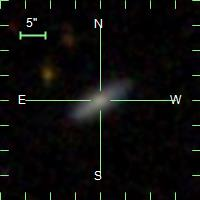
\includegraphics[width=0.25\textwidth]{/home/theo/Учеба/Праки/cosmoprak/example/getjpeg.jpeg}
  \caption{Галактика [Ra, Dec] = [142.762485722253, 28.5431078946331]}
  \label{fig:имя_фигуры}
\end{figure} \\Eго спектр имеет вид:
\begin{figure}[h!]
  \centering
  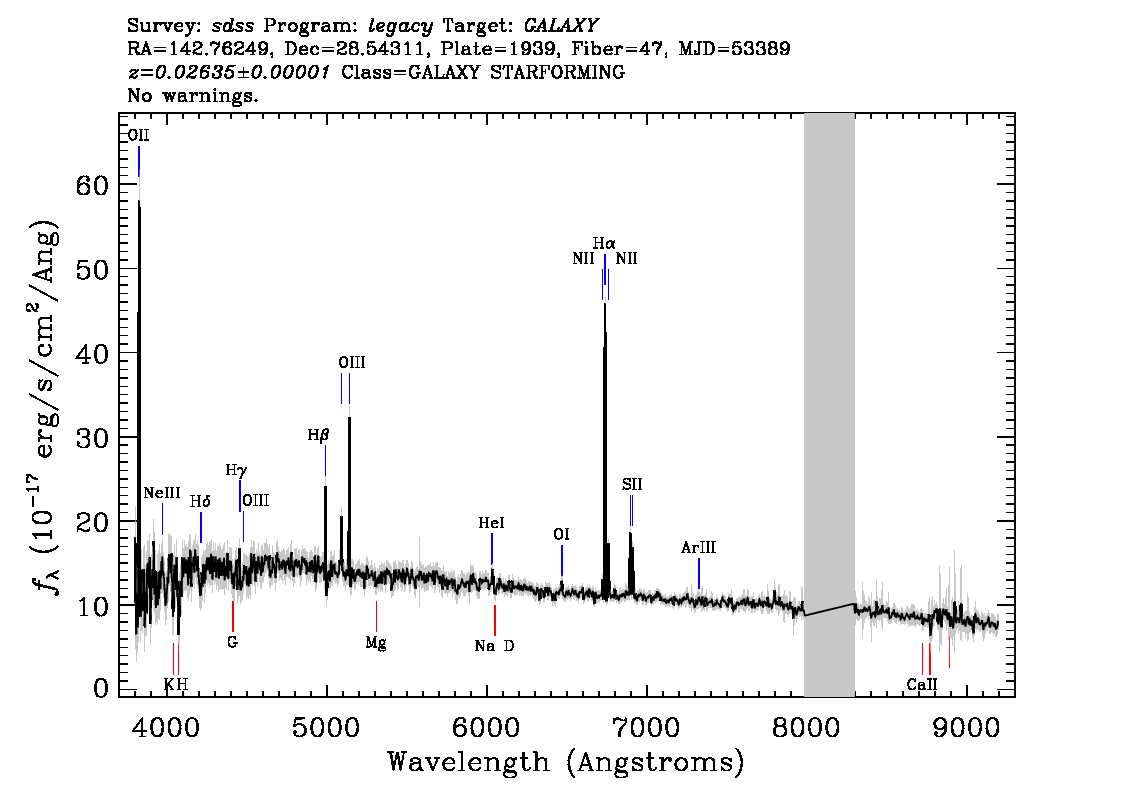
\includegraphics[width=0.75\textwidth]{/home/theo/Учеба/Праки/cosmoprak/example/SpecById.png}
  \caption{Спектр галактики}
  \label{fig:имя_фигуры}
\end{figure}
\\На спектре мы видим различные пики, соответствующие излучению различных элементов. Нас будут 
интересовать линии серии Бальмера $H_\beta$ и дублет $OIII$, поскольку с ними удобно работать. Более
красная линия дублета имеет пик выше, для $O_{III}$ мы будем использовать её. \\\\   
Из таблицы .CSV (не представленной в примере) для данного спектра, мы получим их длины волн:
$$\lambda(H_\beta) = 4991.143 \text{ Å,  }\; \lambda(O_{III})= 5140.436 \text{ Å}$$
В качестве референсных линий можете воспользоваться данными значениями:
\begin{figure}[h!]
  \centering
  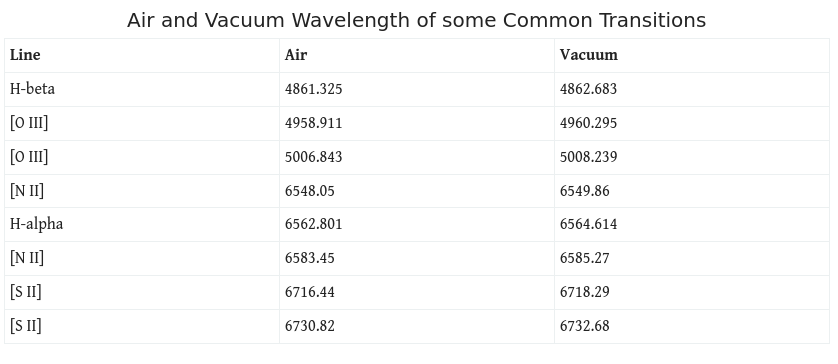
\includegraphics[width=0.9\textwidth]{/home/theo/Учеба/Праки/cosmoprak/example/table1.png}
  \caption{Лабораторные значения длины волн различных линий}
  \label{fig:имя_фигуры}
\end{figure}\\
Таким образом, пользуясь формулой (75), для данной галактики получим:
$$z \approx 0.02639 $$
Особо внимательные студенты могли заметить, что в шапке графика присутствует значение
красного смещения, вычисленное автоматически при создании графика:
$$z = 0.02635 \pm 0.00001 $$
Как видим, мы, пользуясь только калькулятором и спектром, смогли с точностью до 4-го знака после запятой
вычислить красное смещение объекта. Расхождение наших подсчетов с точным значением вызвано
искажением длины волны при прохождении её сквозь атмосферу. Если провести оценку точности,
то, с нашими ошибками, мы можем определить расстояние до объекта с погрешностью в 
несколько сотен тысяч световых лет. В космологических масштабах это очень точное 
измерение - ошибка сравнима с диаметром Млечного пути. \\
\ttt{Задание}:\\
Перейдите по данной ссылке: $$\boxed{\text{\url{https://github.com/BogdanAlenovich/astropractise}}}$$
В данной директории находится 8 таблиц .CSV со спектрами разных объектов.\\\\ \textbf{Вам необходимо}:\\
\textbf{1) Построить графическое изображение спектров}\\
\textbf{2) Отождествить на спектре линии излучения $H_\beta$ и дублета $OIII$}\\
\textbf{3) Вычислить для объекта красное смещение} \\
\textbf{4) Составить таблицу [Номер объекта, $\ff{\lambda(H_\beta)}$, $\ff{\lambda(O_{III}^{right}})$, z]}
\\\\По итогу упражнения необходимо представить: \textbf{графики (8 шт.), таблица (1 шт.)}
\newpage
\subs{Задача 2}
\subsection*{Задача 2: Определение параметров Вселенной в заданный момент времени (\ttt{1 балл})}
Вспомним формулу (27). В качестве соглашения, мы можем принять $a(t_0) = 1$ (нормируем
значения масштабного фактора на его современное значение). \\
Поскольку в данный момент времени мы можем пользоваться приближением Вселенной с
доминированием пыли, по формуле (70) мы можем определить момент времени, в который
был испущен свет от объекта. Для этого произведём тривиальные действия - из (27) получаем:
\eq{\lambda_0 = \frac{\lambda_1}{a(t_1)} \Rightarrow a(t_1)=\frac{\lambda_1}{\lambda_0}}
[\ttt{ВАЖНО}] Не путайтесь: $t_0$ время \ttt{приёма} сигнала, а $t_1$ - время 
\ttt{испускания}. Нумерация произведена в соответствии с логическим порядком: нулевые 
коэффициенты относятся к настоящему времени.  

-------------------------------------------------------------------------------------------------------
--------------------------------------------------------------------------------------------------------------
-------------------------------------------------------------------------------------------------------
--------------------------------------------------------------------------------------------------------------
-------------------------------------------------------------------------------------------------------
----------------------------------------------------вв----------------------------------------------------------
-------------------------------------------------------------------------------------------------------
--------------------------------------------------------------------------------------------------------------
-------------------------------------------------------------------------------------------------------
--------------------------------------------------------------------------------------------------------------
-------------------------------------------------------------------------------------------------------
--------------------------------------------------------------------------------------------------------------
-------------------------------------------------------------------------------------------------------
--------------------------------------------------------------------------------------------------------------
-------------------------------------------------------------------------------------------------------
--------------------------------------------------------------------------------------------------------------
-------------------------------------------------------------------------------------------------------
--------------------------------------------------------------------------------------------------------------
-------------------------------------------------------------------------------------------------------
--------------------------------------------------------------------------------------------------------------
-------------------------------------------------------------------------------------------------------
--------------------------------------------------------------------------------------------------------------
-------------------------------------------------------------------------------------------------------
--------------------------------------------------------------------------------------------------------------
-----------------------------------------------------------------------------
=============================================================================================================
=====================================================================================================
=============================================================================================================
=====================================================================================================
=============================================================================================================
=====================================================================================================
---------------------------------------------------------------------ЧЕРНОВИК-----------------------------
\\\\\\\\\\\\\\\\\\\\
\\Подставляя в (70), получим:
\eq{\frac{\lambda_1}{\lambda_0}=\left(\frac{t_1}{t_0}  \right)^{\frac{2}{3}}}
Преобразовывая, находим время:
\eq{t_1 =t_0 \sqrt{\left( \frac{\lambda_1}{\lambda_0} \right)^3} }
Теперь посчитаем, какое расстояние прошёл свет с момента, когда его испустила галактика. 
Считая скорость света постоянной в каждой точки пути, получим:
\eq{L = c \Delta t = c\left( t_0 - t_1 \right)=\left( 1 - \sqrt{\left( \frac{\lambda_1}{\lambda_0} \right)^3} \right)ct_0}
Если пользоваться переводом отношения длин волн в красное смещение:
\eq{1+z = \frac{1}{a(t_1)}}
то, мы получим:
\eq{L = \left(1-\sqrt{\frac{1}{(1+z)^3}}\right)ct_0}
\ttt{--- разобраться в расстоянии-------------------------}

\newpage
\end{document}

